\documentclass[tikz, border=5pt]{standalone}

% Librerie TikZ
\usepackage{tikz}
\usetikzlibrary{
    arrows.meta,        % frecce moderne
    calc,               % calcoli con coordinate
    positioning,        % posizionamento avanzato dei nodi
    shapes.geometric,   % forme (rettangoli, cerchi, diamond, ecc.)
    shapes.misc,
    decorations.pathmorphing,
    patterns
}

% Opzionale: font coerente con il documento principale
\usepackage{lmodern}

\begin{document}

    %  figura tikz
    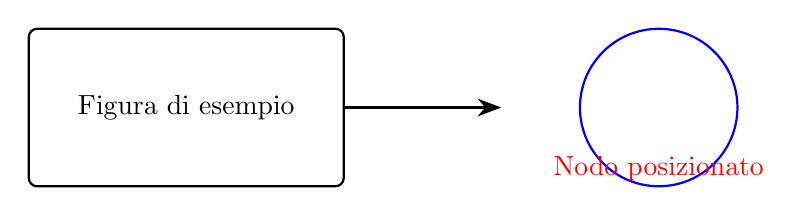
\begin{tikzpicture}

        % Esempio: rettangolo con testo
        \draw[thick, rounded corners=3pt] (0,0) rectangle (4,2);
        \node at (2,1) {Figura di esempio};

        % Esempio: freccia moderna
        \draw[-{Stealth[length=3mm]}, thick] (4,1) -- (6,1);

        % Esempio: cerchio
        \draw[blue, thick] (8,1) circle (1);

        % Esempio: nodo posizionato
        \node[red, below=5mm of {(8,1)}] {Nodo posizionato};

    \end{tikzpicture}
\end{document}

